
\section{Results}

The model was tested in several scenarios. First, the price 
dynamics and order book evolution are studied with a simple one market settings in which the dividend
yield and interest rate are set to zero. Then the same aspects are investigated
using more complex settings: only some of the traders are allowed to place orders
per trading session and the dividend yield and interest rate are set to random walk.
Then arbitrage is studied using 
a setting in which there exists two identical markets.


\subsection{Single asset simulation}
% Price dynamics, stylized facts, order book evolution
The single asset simulation was run twice: first run
was conducted with a starting market price of 500 and second
with a starting market price of 1500. The simulations were
run with 500 traders trading 1000 rounds. The 
amount of currency and the amount of stock 
a trader owns in the beginning of the simulation were set to
10 000 000 and 10 000 respectively. Therefore
the ratio of stock to currency is 1 000 which
is the expected equilibrium price as there are
no payouts in either asset. The amount of currency
per trader may seem much but as the tick size is one,
it may be more convenient to think the currency in amounts
in cents or pennies. The standard deviation of
the price each trader bids and asks with is set to 20. The 
starting market price was set to 400 to study the 

% Descriptive analysis
The evolution of trade prices, quantities and values thorough
the trading sessions for both simulations are shown in the figure
~\ref{fig:basic_trades}. As can be observed,
the near equilibrium market price is achieved in around 20 trading
sessions for both runs. The reason why the price stays slightly 
under the equilibrium price may be caused by the implementation of
determining the order price and order quantity. If a trader decides
to allocate less currency on an order than the decided order price 
the order gets obviously invalidated but there is no such
limitation for placing asks. Therefore there might be a slightly less
bids than asks in general. 

\begin{figure}
    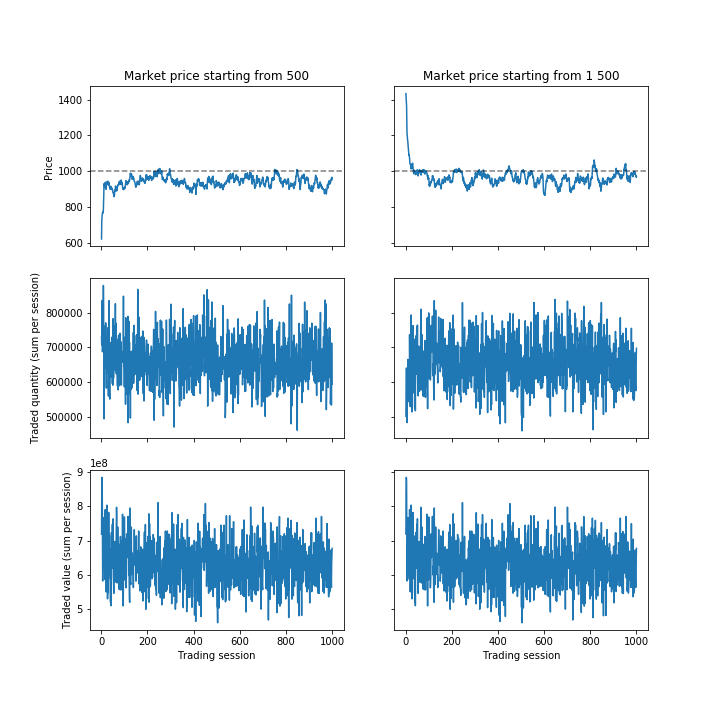
\includegraphics[width=\linewidth]{plots/basic_trades.png}
    \caption{Evolution of price and quantity}
    \label{fig:basic_trades}
\end{figure}

% How the market converged to equilibrium
The market depths shown in figure ~\ref{fig:market_depths} suggests that the
converge to equilibrium is caused by balancing the sides of the market. 
In the figure the order book is visualized for the first 100 trading sessions. 
The surface describes the evolution of the cumulative bids and cumulative asks 
thorough time and the bottom of the valley in the surface is the bid-ask spread. 
The left side from the valley is the the bid book and the right is the ask book. The 
ask side of the market is almost completely missing initially in the run that
starts with lower market price while the opposite is true for the run with higher
initial market price. The side emerges rapidly after few trading session
and the market price approaches near equilibrium price and vice versa for the 
simulation starting with higher market price. An example of the market depth 
when the equilibrium is reached is shown in ~\ref{fig:basic_market_depth_equilibrium}.


\begin{figure}
    \centering
    \begin{subfigure}{.5\textwidth}
      \centering
      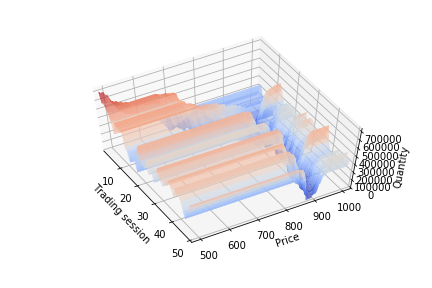
\includegraphics[width=\linewidth]{plots/basic_market_depth_converge_lower.png}
      \caption{Starting price 500}
      \label{fig:market_depth_lower}
    \end{subfigure}%
    \begin{subfigure}{.5\textwidth}
      \centering
      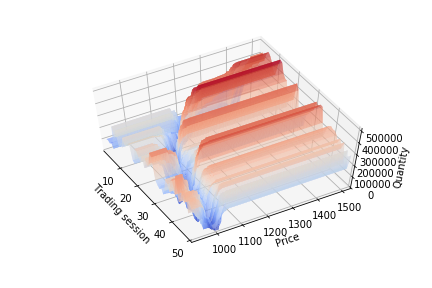
\includegraphics[width=\linewidth]{plots/basic_market_depth_converge_higher.png}
      \caption{Starting price 1 500}
      \label{fig:market_depth_higher}
    \end{subfigure}
    \caption{Converge of the order book to equilibrium}
    \label{fig:market_depths}
\end{figure}

% Evolution and characteristics of the order book via the heatmap
The complete evolution of the order book thorough the simulations is shown in figure
~\ref{fig:basic_orderbook_evo}. The 

\begin{figure}
    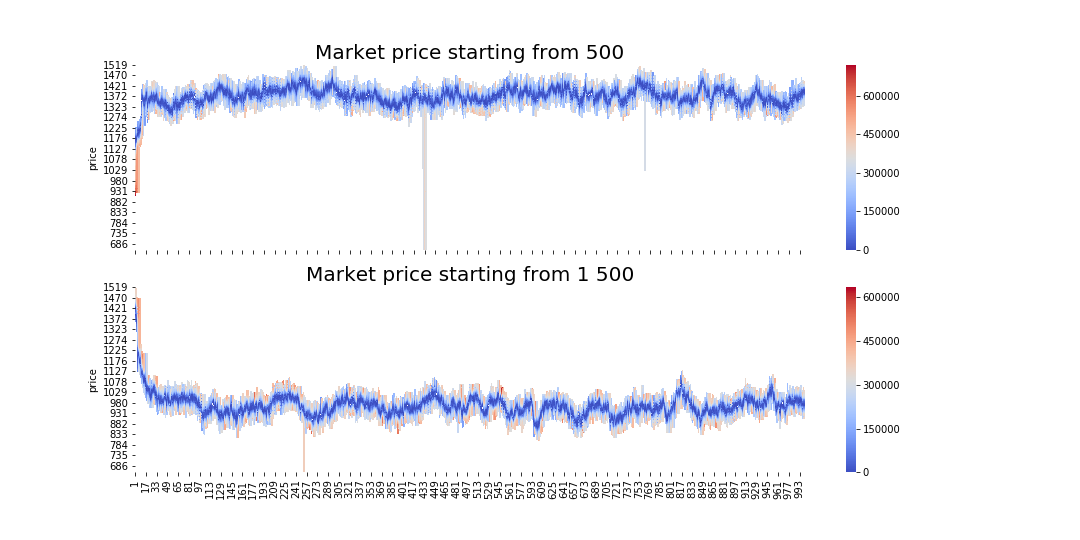
\includegraphics[width=\linewidth]{plots/basic_order_book_evo.png}
    \caption{Order book evolution}
    \label{fig:basic_orderbook_evo}
\end{figure}


\begin{figure}
    % Probably remove this
    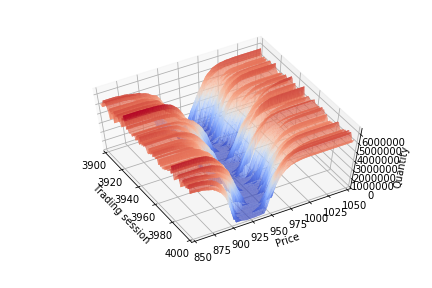
\includegraphics[width=\linewidth]{plots/basic_market_depth_in_equilibrium.png}
    \caption{Market depth when equilibrium reached (last 50 sessions)}
    \label{fig:basic_market_depth_equilibrium}
\end{figure}

% stylized facts
% Somethging about filtering fist 100 out and now inspecting stylized facts
As stated before, the representativeness of real markets is inspected using
stylized facts. In order to have represenative data set to test the facts, the
sessions before reaching the price equilibrium are filtered out. 
As observed in ~\ref{fig:basic_trades}, the model reaches the equlibrium 
price before the 100th trading session and after that both of the initiations 
yield similar price and quantity processes. Therefore, for simplicity the
the first 100 trading sessions are filtered out from the simulation with
lower initiated market price and the data produced from it is used for 
studying the stylized facts in the model.

% Autocorrelation
The autocorrelation function (ACF) and partial autocorrelation function (PACF) for the last prices of
each session are plotted in the figure ~\ref{fig:basic_autocorr}. Even though the literature discuss
about the absence of autocorrelation in asset returns, the prices themselves are already stationary when
the equilibrium is reached which is obviously not the case in real markets. ACF and PACF indicate that there is 
an autoregressive (AR) process for up to 15 lags and a moving average (MA) process to the third lag. Therefore
there is a clear autocorrelation in the model with the stated simulation parameters. One could expect such
a behaviour to be caused by the traders' option of not changing their active order which happened with a probability of
one-third per placement. As the price in each order
is dependent on the market price which existed when the order was created and as there is a chance that
this order will stay in the order book for some time, therefore the market price in the past has influence on the
current structure of the order book as some of the orders are carried to future state of the market. 
In other words, a past market prices may have effect on the upcoming prices via the order book.
This phenomenon can be interpret from the figure ~\ref{fig:basic_market_depth_equilibrium}: the valley
formed by the sides of the order book resembles river.

\begin{figure}
    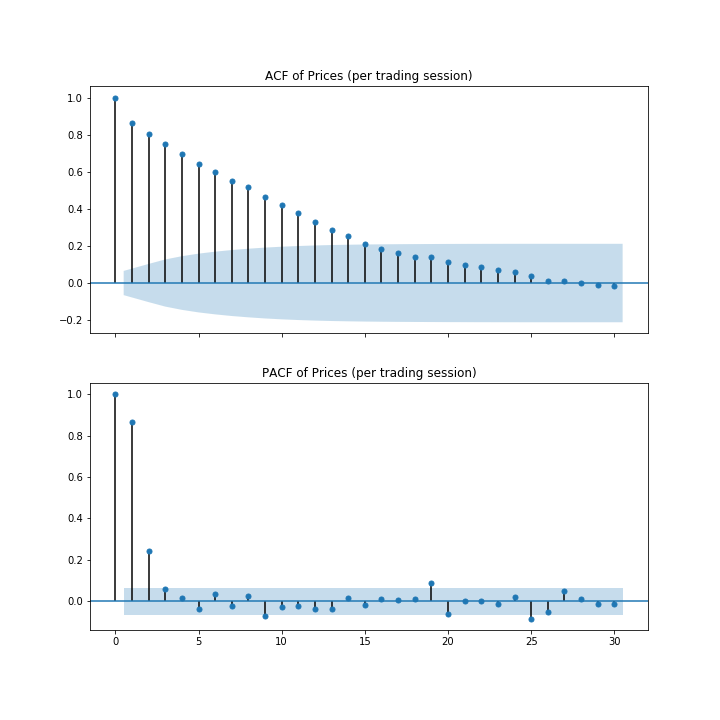
\includegraphics[width=\linewidth]{plots/basic_autocorrelation.png}
    \caption{Autocorrelation of the simulation after 100 session}
    \label{fig:basic_autocorr}
\end{figure}

% The real reason for the autocorrelation
However, this is not the underlying reason for the existence of the autocorrelation. There is similar type and
magnitude of autocorrelation when the option of doing nothing is taken away. This can be observed in the figure 
~\ref{fig:forcesub_autocorr}. This suggests that the autocorrelation is not caused by the order book structure
as in the said experiment the order book reconstructed during each session. Furthermore, as the investors themselves are
not aware of the past and only their positions are the only component reflecting the past, explanation for the 
autocorrelation lies in these positions. Even though the total amount of currency and stock stay constant throughout
trading sessions the distribution of the assets among the traders do not. The relationship between the imbalance
of the assets between the traders, represented as the standard deviation of the positions among the traders, and
the next session's last market price is studied using a multivariate linear regression. This model's performance is
shown in the table ~\ref{tbl:price_explanation}. The model is statistically significant as the p-value of f-statistics
is near zero. In addition, the coefficient of determination, called R squared, is as high as 0.999 meaning that
almost all of the variance in the next session's price is explained by the regression model. To summarize, the
autocorrelation is caused by the imbalance of the positions among the traders and not by the market microstructure
or as a direct result of the decision mechanics of the traders. There is significant multicollinearity in the regression
model thus the individual coefficients or the p-values of the explanatory variables cannot be interpret but this 
does not as is affect to the predictability of the model. 


\begin{figure}
    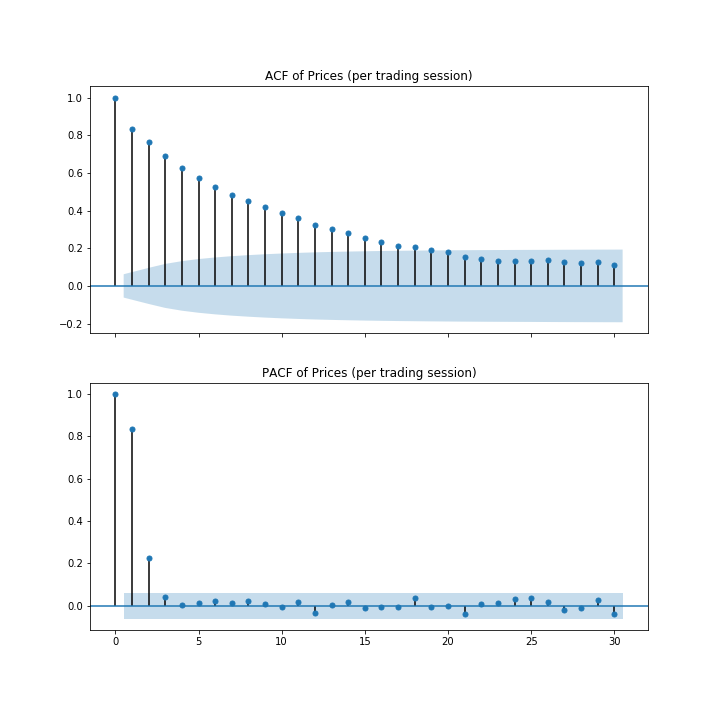
\includegraphics[width=\linewidth]{plots/forcesub_autocorrelation.png}
    \caption{Autocorrelation of the simulation of no option for inaction}
    \label{fig:forcesub_autocorr}
\end{figure}

\begin{table}
    \begin{center}
\begin{tabular}{lclc}
\toprule
\textbf{Dep. Variable:}                            & Last price per session, shifted 1 & \textbf{  R-squared (uncentered):}      &     0.999   \\
\textbf{Model:}                                    &                OLS                & \textbf{  Adj. R-squared (uncentered):} &     0.999   \\
\textbf{Method:}                                   &           Least Squares           & \textbf{  F-statistic:       }          & 5.924e+05   \\
\textbf{Date:}                                     &          Mon, 22 Jun 2020         & \textbf{  Prob (F-statistic):}          &     0.00    \\
\textbf{Time:}                                     &              21:47:20             & \textbf{  Log-Likelihood:    }          &   -4731.1   \\
\textbf{No. Observations:}                         &                  999              & \textbf{  AIC:               }          &     9466.   \\
\textbf{Df Residuals:}                             &                  997              & \textbf{  BIC:               }          &     9476.   \\
\textbf{Df Model:}                                 &                    2              & \textbf{                     }          &             \\
\bottomrule
\end{tabular}
\begin{tabular}{lcccccc}
                                                   & \textbf{coef} & \textbf{std err} & \textbf{t} & \textbf{P$> |$t$|$} & \textbf{[0.025} & \textbf{0.975]}  \\
\midrule
\textbf{Std Dev of currency positions per session} &       0.0002  &      3.8e-06     &    50.178  &         0.000        &        0.000    &        0.000     \\
\textbf{Std Dev of stock positions per session}    &      -0.0515  &        0.004     &   -14.215  &         0.000        &       -0.059    &       -0.044     \\
\bottomrule
\end{tabular}
\begin{tabular}{lclc}
\textbf{Omnibus:}       & 13.010 & \textbf{  Durbin-Watson:     } &    0.865  \\
\textbf{Prob(Omnibus):} &  0.001 & \textbf{  Jarque-Bera (JB):  } &   21.220  \\
\textbf{Skew:}          &  0.002 & \textbf{  Prob(JB):          } & 2.47e-05  \\
\textbf{Kurtosis:}      &  3.714 & \textbf{  Cond. No.          } & 2.88e+04  \\
\bottomrule
\end{tabular}
%\caption{OLS Regression Results}
\end{center}

Warnings: \newline
 [1] Standard Errors assume that the covariance matrix of the errors is correctly specified. \newline
 [2] The condition number is large, 2.88e+04. This might indicate that there are \newline
 strong multicollinearity or other numerical problems.% table.tex > \mytable
    \caption{Linear regression explaining future price with the Standard deviation of stock and currency positions per session}
    \label{tbl:price_explanation}
\end{table}

% Proposion to real markets
This finding also has a proposion for real markets: the price may also be driven by the imbalance of wealth between traders 
not just the total amounts of assets. For example, if one buyer has excess cash compared to other investors that buyer is more 
inclined to make a bid order of higher value than others. This buyer has an option to overshoot the price by buying 
significant block of the ask side increasing the market price rapidly but this kind of burst less likely if the cash 
is equally distributed among the buyers and the buyers make decisions independently. In the latter case there is less
impact for each buyer to the market price thus such burst of price would require coordination between the buyers.

% How to fix autocorrelation
To reduce the autocorrelation, one option would be to increase the amount of traders to dilude the effect as then
one trader skewing their positions has little impact on the price dynamics. Another option would be to change the 
distribution or logic how the traders pick amount of currency and stock to allocate to each order.In addition, 
\citet{StylizedFacts01} also discussed that also the real markets may have some autocorrelation 
of returns for small intraday time periods, such as 20 minutes, and therefore one trading session in the simulation 
may be more closer, in terms of comparison, to an intraday time period. However, they stated this autocorrelation
to be caused by market microstructure and as this could be also a cause in the autocorrelation in the simulation,
the more impactful component is the asset imbalance with current simulation parameters and implementation.


% Fat-tailed returns
In order to increase the robustness of estimating whether the market prices have fat tails or not, the parameters of the
simulations are left unchanged except that the simulation is extended to 10 000 sessions. Jarque-Bera goodness of fit test,
which was used to determine if the distributions are normal or not, require substantial sized sample in order to be accurate.
The null hypothesis of Jarque-Bera test is a joint hypothesis of that the distribution has no skewness and excess kurtosis. 
As can be observed from ~\ref{fig:basic_return_distr_per_session} and ~\ref{fig:basic_return_distr_intrasession}, the last 
prices of sessions are normally distributed but not the intrasession prices. The p-values of Jarque-Bera test suggests similar
results: 0.73 and 0.00 respectively. Therefore the null hypothesis is rejected for the intrasession returns but not for
end of session returns. This is inline with the findings of \citet{Raberto05}. However \author{Raberto05} had slightly
different market structure: their model's order book was emptied after each trading day and ...
\author{Raberto05} did not discuss about the fat tailed returns more than that they are formed due to the market microstructure.
The spike in the distribution of the intrasession returns may be caused by the structure of the order book. If the order book 
sides are steep, as observed in this simulation illustrated in ???, it requires substantially sized order to push the opposing 
side back and have a significant effect on the price. Therefore the price changes between trades are generally rather small
until there comes an order that can buy or sell significant chunk of the opposing side and have instant impact on the price. 
In such a case the opposing side may be weakened so much that the price change can be radical. Therefore the reason for the
spike in the returns may be caused by the occurence that small and medium sized orders may have similar impact on the price
but big orders may push the side relatively much more further as the density of the order quantitity drops when moving further
away from the last market price.


The returns of the market prices after each session are not fat-tailed distributed as can be observed from the figure 
~\ref{fig:basic_return_distr_per_session} but the intrasession . This is somewhat expected: the order prices themselves are drawn from a normal distribution.
However, the returns between trades do diverge from normal distribution, as can be observed ~\ref{fig:basic_return_distr_intrasession} 
from  but this occurs due to the effects the of microstructure in short term. If one order has high quantity and 
relatively attractive price the order might get matched multiple times in a row resulting in the spike of zero return 
shown in the figure. One option to produce the fat-tailed distributions could be to shift the mean of the normal distribution, 
which is used to draw the order prices, depending on whether the order is a bid or an ask. 

% \citet{Raberto05} found fat tails in intra day


\begin{figure}
    \centering
    \begin{subfigure}{.5\textwidth}
        \centering
        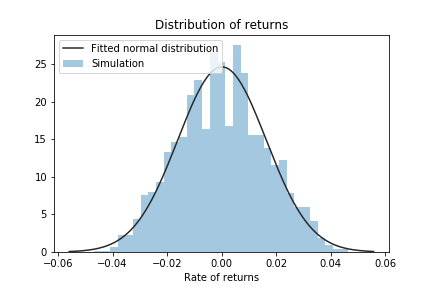
\includegraphics[width=\linewidth]{plots/basic_fat_tails_per_session.png}
        \caption{Last price of each session}
        \label{fig:basic_return_distr_per_session}
    \end{subfigure}%
    \begin{subfigure}{.5\textwidth}
        \centering
        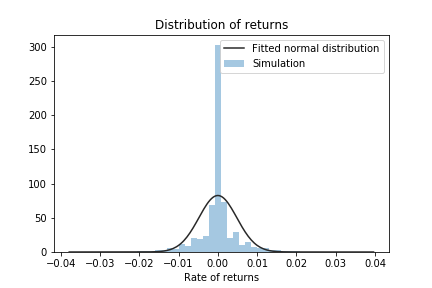
\includegraphics[width=\linewidth]{plots/basic_fat_tails_intrasession.png}
        \caption{Between trades}
        \label{fig:basic_return_distr_intrasession}
    \end{subfigure}
    \caption{Distributions of returns after 100 sessions}
    \label{fig:basic_return_distr}
\end{figure}


% Volatility clusters
The autocorrelation of the volatilities in figure ~\ref{fig:basic_volaclusters}
indicate there are some volatility clusters in short term. Both, ACF and PACF, shows slow
decay indicating that there are both of the autocorrelation terms, AR and MA,
present in the volatility of the market price. The effect is, however, rather short term
as it is not carried over trading sessions as shown in the appendix ~\ref{app:basic_volaclusters_per_session}.


\begin{figure}
    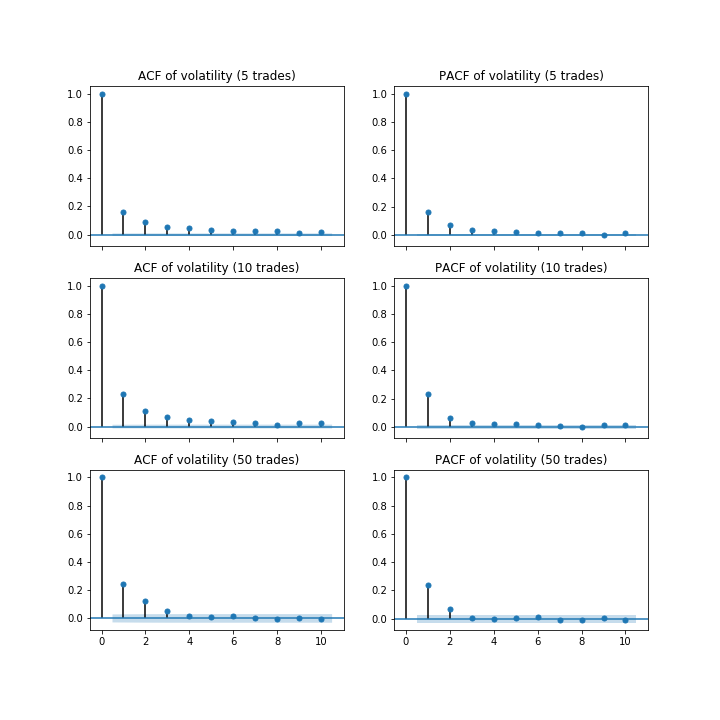
\includegraphics[width=\linewidth]{plots/basic_volaclusters_intraday.png}
    \caption{Volatility Clusters}
    \label{fig:basic_volaclusters}
\end{figure}

\subsection{Arbitrage simulation}

To contribute to 
